\documentclass[a4paper]{article}


\usepackage[T1]{fontenc}    
\usepackage[utf8]{inputenc} 
\usepackage{textcomp}      
\date{} 					
\author{}                   
\usepackage{geometry}		
\geometry{ left=2cm, right=2cm, top=2cm, bottom=4cm, bindingoffset=5mm}

\usepackage{graphicx}
\usepackage{xcolor}
\usepackage{hyperref} 
\usepackage{fancyhdr}												
\pagestyle{fancy}
\fancyhf{}
\fancyhead[R]{2973140 - Felix Bühler  \\ 2893121 - Jan Leusmann \\  3141241 - Jamie Ullerich}
\fancyhead[L]{Scientific Visualisation \\ Sommersemester 2019 }
\renewcommand{\headrulewidth}{0.5pt} 				

\title{Exercise 5}

\begin{document}
	
	\maketitle 
	\thispagestyle{fancy}
	

	
	\section*{Exercise 5. 1 [3 Points] Delaunay Triangulation - Edge-Flip}
	
	\begin{figure}[h!]
		\centering
		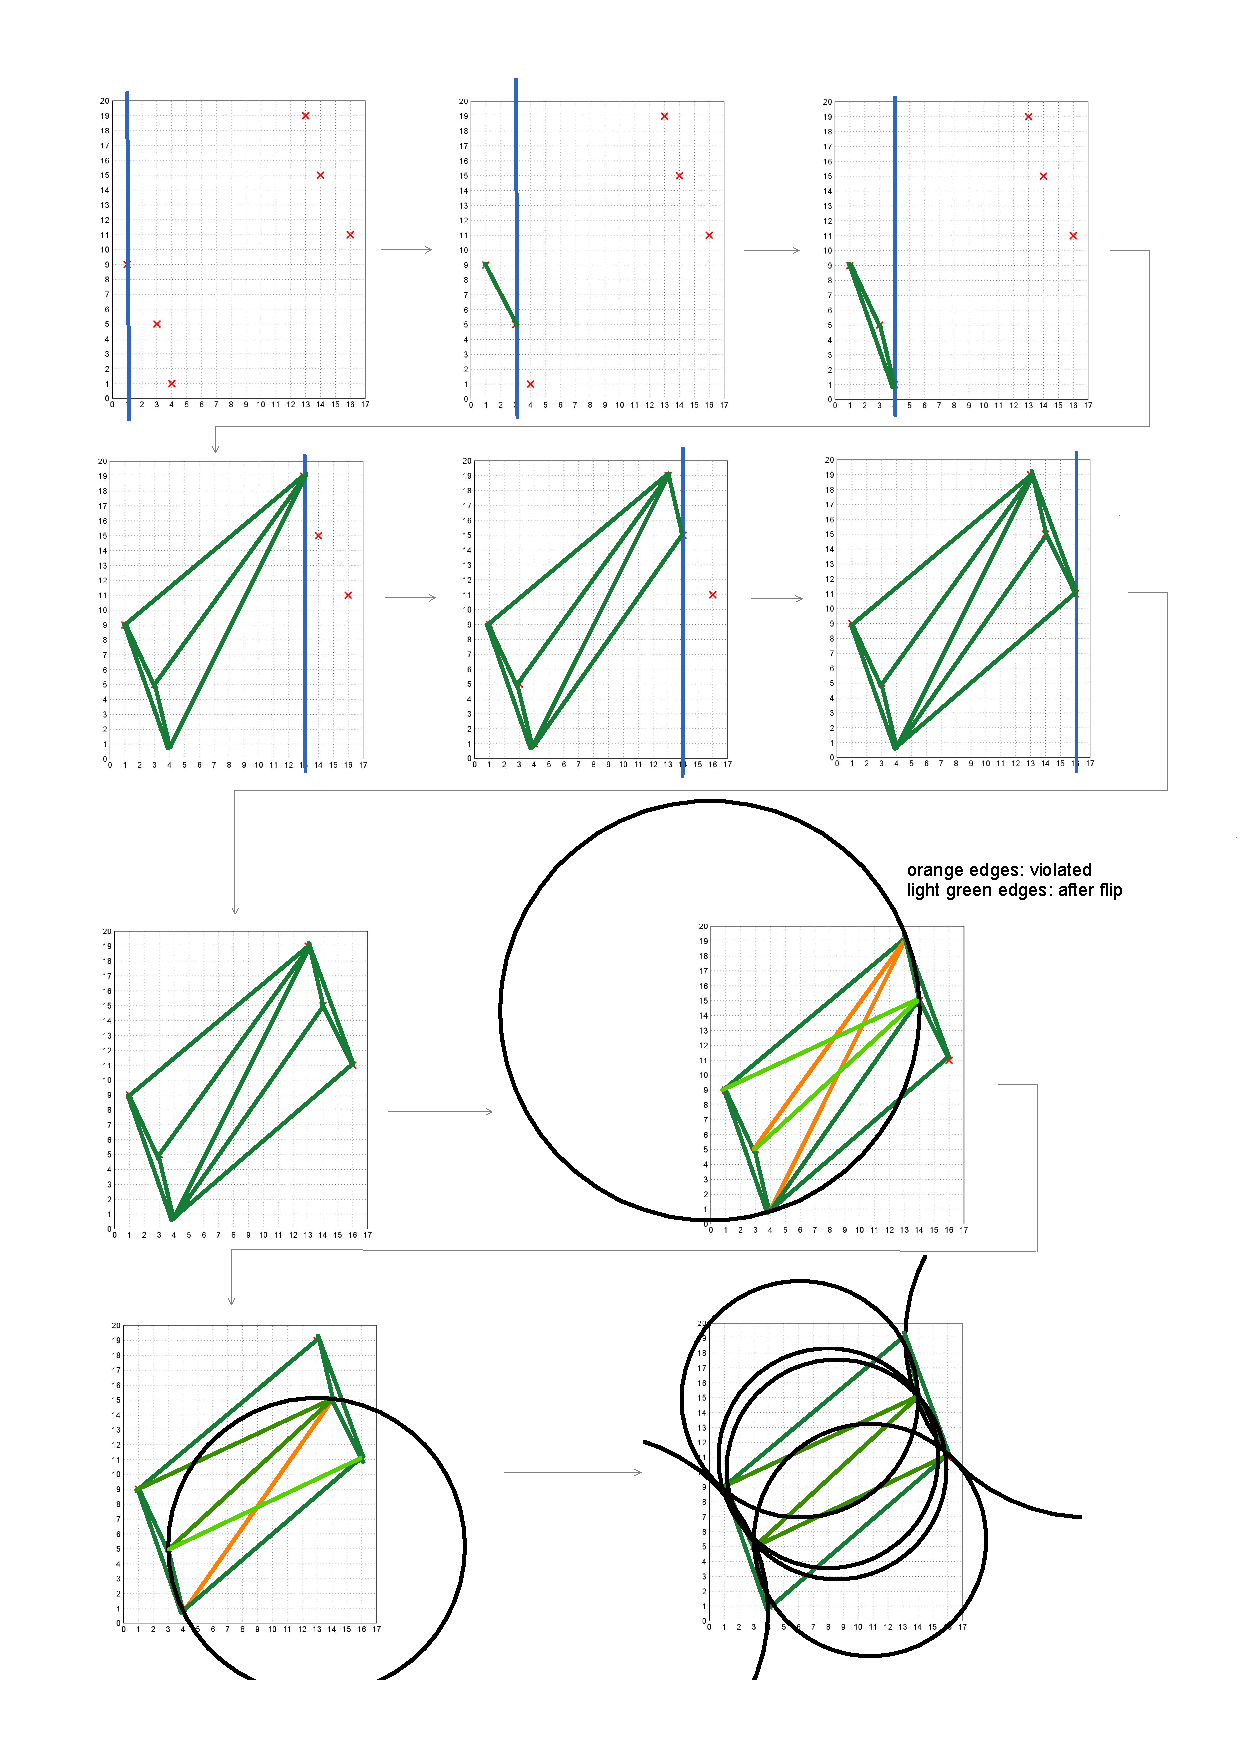
\includegraphics[width=0.79\linewidth]{delaunay.pdf}
		%\caption{}
		\label{fig:diagram}
	\end{figure}

	\clearpage
	
	\section*{Exercise 5. 2 [3 Points] Inverse Distance Weighting}
	

	

	
	
	
	\section*{Exercise 5. 3 [1 Points] Interpolation inside a prism}
	
	
	
	\section*{Exercise 5. 4 [5 Points] Paraview: Simple Gradient Plugin}
	
	
	
\end{document}